\section{Machine Learning based Method}

\TODO{Twitter API for test data?}
\subsection{Training data}
The training data for machine learning classifiers was created by Go et al. and consists of 1.6 million tweets \cite{GoBHaHua2009}. The tweets were parsed using the Twitter API by querying for positive or negative emoticons, such as ":)" and labeled as positive or negative depending on the emoticon. Furthermore, tweets containing both a negative and positive emoticon, as well as retweets were removed \cite{GoBHaHua2009}.

This resulted in 800,000 positive and 800,000 negative tweets that were periodically requested on no specific topic, thus covering a huge amount of topics \cite{GoBHaHua2009}.
\TODO{put bi-gram and stemming + filtering, etc. in Methodology --> general Workflow for ML, here: numWords, LowerCase, Occurences, LovinsStemmer, bigram...}
\TODO{some sources, why..., 79.8853 \%}
\subsection{Preprocessing}
Before classifying can begin, tweets must be preprocessed. Because every word is treated as an attribute, some words can be removed in advance to improve both accuracy and performance \TODO{STOP WORDS = the...}. This includes frequent words such as "is", "I", and "the", which do not affect the sentiment of a tweet and can therefore be ignored. Finally, every word is transformed to lower case to prevent case sensitity, in addition to URLs being removed. Weka uses the Attribute-Relation File Format for its data, which contains a header describing the attributes, as well as the data itself, with one row containing one instance \cite{weka}. For this thesis, the class attribute was chosen to be nominal, either negative (-1.0) or positive (1.0), so we have a binary classification problem. Furthermore, the tweet text is added as a string attribute.

\subsection{Filtering}
In order to transform the text of a tweet into a suitable format for classifiers, weka's StringToWordVector filter is used \cite{weka}. This filter transforms the string feature, the tweet's text, by parsing each word out of it. The words are then added to a dictionary, which stores all recognized words. In the data, the words are implemented as numeric attributes, with the value denoting the number of occurrences.

For example, the tweet "i love it" would result in three attributes, the attribute "i", the attribute "love", and the attribute "it", as can be seen in Figure \ref{fig:arff_train}. The dictionary, and with it the attributes, are all determined by the training data. The test data are also filtered, but only using the known words from the training data, no new words are added. 


Additionally, a bi-gram model was used, which allows an attribute to consist of up to two words. Doing so allows us to replicate certain important relationships between two words, such as "not good". In an uni-gram model, each word is looked at separately, which results in the loss of "not" negating the positive "good". By using "not good" as a feature, the negation is taken into account and the attribute is thus clearly negative.

If every word/bi-gram was used as an attribute, the attribute size would be enormous and thus lead to performance problems. To prevent this, a limit was set for how often a word has to appear to be used as well as a (soft) limit of total words. In the testing, a limit of 15,000 words was found to be optimal, with words appearing at least 20 times in the training data.
\TODO{source}

Furthermore, the number of available words can be further reduced by using word stemming, which, according to Lovins, "reduces all words with the same root (or, if prefixes are left untouched, the same stem) to a common form" \cite[p.~22]{Lovins1968DevelopmentOA}. It does this using a two-step method, which first removes the ending, thus resulting in the stem. After this, similar stems are combined to account for different spellings. An example for this is "absorption", whose stem is "absorpt", while "absorbing" will result in "absorb". By using word stemming, related words are matched, thus creating combined attributes instead of considering each word form to be separate.

 
\begin{figure}
    \centering
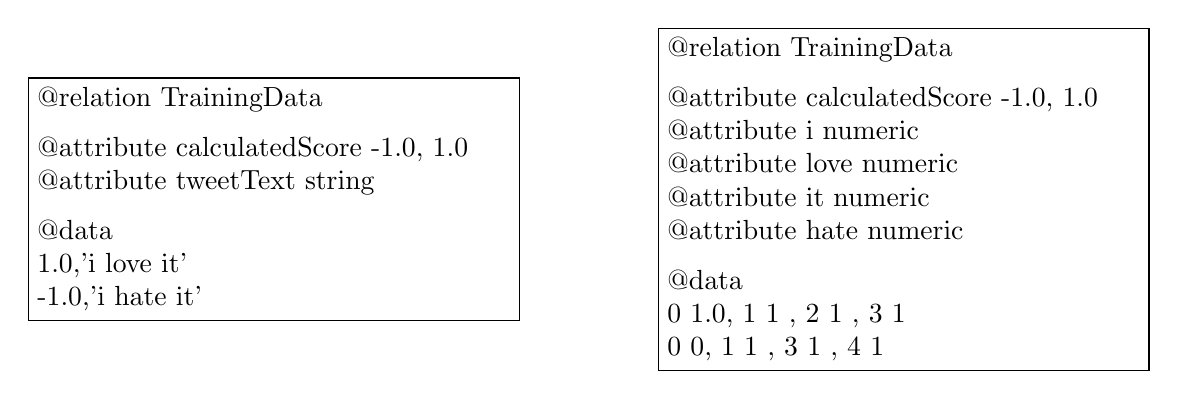
\begin{tikzpicture}
\node[draw, text width=6cm] at (0,0) { @relation TrainingData \\
                                        \medskip
                                        @attribute calculatedScore {-1.0, 1.0} \\
                                        @attribute tweetText string \\
                                        \medskip
                                        @data \\
                                        1.0,'i love it' \\
                                        -1.0,'i hate it' \\
                                        
                                        };
\node[draw, text width=6cm] at (8,0) { @relation TrainingData \\
                                        \medskip
                                        @attribute calculatedScore {-1.0, 1.0} \\
                                        @attribute i numeric \\
                                        @attribute love numeric \\
                                        @attribute it numeric \\
                                        @attribute hate numeric \\
                                        \medskip
                                        @data \\
                                        {0 1.0, 1 1 , 2 1 , 3 1} \\
                                        {0 0,   1 1 , 3 1 , 4 1}
                                        };
\end{tikzpicture}
    \caption{Caption}
    \label{fig:arff_train}
\end{figure}

\begin{itemize}
    \item StringToWordVector
    \item Amount of words + dictionary
    \item Occurences minimum
    \item N-Gram?
    \item 79.4226 with lovinsstemmer
    \item lowercase
    \item Binary vs. NumWords
    \item ARFF
\end{itemize}
\subsection{Training}
\begin{itemize}
    \item Comparison Classifiers --> Accuracy? Runtime (Complexity), 78.60
    \item ARFF
    \item maybe experiment with number of training tweets?
    \end{itemize}
\TODO{Where improvements to filtering?}

Once the training data has been preprocessed and filtered, the actual task of training the models can begin. As previously discussed, the classifiers chosen were Naive Bayes using the Gaussian Distribution, Naive Bayes using the multinomial Distribution, Random Forest, Logistic Regression and Support Vector Machine. The process for each classifier can be described as follows: First, the classifier was trained using the standard parameters set by Weka and a small subsection of the training data (\~12,000 tweets). This was done to provide a first impression of the training runtime, which proved to have a great effect. After this, the subset of training data was gradually increased, until the entire data set was used, or the process became too resource intensive. Once the appropriate training size was found, the parameters of each classifier were evaluated, both to improve performance and accuracy. If performance was improved, the training size was also increased accordingly.

\subsection{Evaluation}
In Table \ref{tab:evaluations}, each classifier can be seen with the optimal parameters, the number of training instances used, and the evaluation parameters discussed.

\begin{table}[]
\centering
\caption{Table to test captions and labels.}
\begin{tabular}{ |p{3cm}||p{3cm}|p{2cm}|p{2cm}|p{2cm}|p{2cm}|  }
 \hline
 Classifier name &          Parameters &             Training Instances &    Accuracy &      Kappa &     Relative absolute error \\
 \hline
 Naive Bayes (Gauss)        &-&            TODO&                 60.99\%&        0.21&       82.14\%\\
  \hline
 Naive Bayes (Multinomial)  &-&                     1231862&                78.67\%&        0.51&       52.22\%\\
  \hline
 Random Forest              &depth = 300&            12318&                 75.48\%&        0.45&       81.33\%\\
  \hline
 Logistic Regression        &iterations = 10&            94655&                 77.40\%&        0.47&       59.70\%\\
  \hline
 Support Vector Machine     &kernel = linear&            TODO&                 77.11\%&        0.48&       45.52\%\\
 \hline
\end{tabular}
\label{tab:evaluations}
\end{table}



